\chapter{NAT}
プロキシの概念は、クライアントに対してはサーバとして振る舞い、サーバに対してはクライアントとして振る舞う中間者、ということでした。では、その概念をインターネットプロトコル層に持ち込んだらどうなるでしょうか。

このアイディアがRFC2663としてまとめられたのは、1999年のことです。
今度は、インターネットプロトコル層でのプロキシといえる、NATについて説明しましょう。

\section{インターネットプロトコル層のプロキシ}
インターネットプロトコル層のプロキシとはどんなものと考えればいいだろうか。これまでのプロキシの定義で考えると、内部のホストからは、別のネットワークにアクセスするためのゲートウェイに見える、そのホストがアクセスする先のホストから見れば、レスポンスを返す先に見える何かである。

まず、LAN側のホストにはプライベートのIPアドレスが割り当てられているとする。この状態では、LANの中のホストはインターネットにアクセスできない。アクセスさせる方法として、プロキシを用意する方法がある。だが、プロキシは特定のアプリケーション層のサービスにしかアクセスできない。任意のインターネットプロトコル上の通信には対応できない。

そこで、任意の通信を行う手段として、IP層でのプロキシを考えてみよう

\section{アクセスとアドレス変換}。
インターネットプロトコル層のプロキシは、どのような動作をすれば良いだろうか。種明かしをすれば、プロキシ役を受け持つ機器が、グローバルのIPアドレスと、プライベートのIPアドレスしかもたないホストのどちらと持つシンができるようにすることである。

この、インターネット層のプロキシは、内部からはただのゲートウェイに見えていなければならない。これは、クライアントから見たとき、ルータとして振る舞っているように見えるという事である。そこで、この先はこのプロキシ役のホストがルータであるとして説明を行う。

\subsection{中から外への通信}

プライベートのIPアドレスしか持たないホストから発信されたIPデータグラムは、まずゲートウェイであるルータに到達する。通常であれば、ルータは」TTLだけ減らしてそのデータグラムを次の宛先に転送する。

だが、届いたIPデータグラムの発信元フィールドは、プライベートなIPアドレスだ。このままインターネットに送出しても、インターネットの先にあるホストは、返信をすることができない。

プロキシ役をするルータはこのIPデータグラムのヘッダの発信元を、自分に割り当てられているグローバルのIPアドレスのひとつに書き換え、転送する。書き換えるIPアドレスは、内部のホストの、プライベートなIPアドレスと一対一対応させる。そのため、書き換え用のIPアドレスは、内部でインターネットアクセスをするホストの数だけ用意する運用が多い。

ただし、このとき、ペイロードがTCPのセグメントやUDPデータグラムであった場合、ペイロードのヘッダのチェックサムを再計算して、再構成しなければならない。
トランスポート層ではIPアドレスの情報を含む疑似ヘッダを用いたチェックサム計算で、セグメント、もしくはUDPデータグラムの破損をチェックするためだが、発信元のIPアドレスが変更されることで、チェックサムの値が、トランスポート層のヘッダ情報に書かれているものとちがうものになってしまう。
そのため、トランスポート層のチェックサムをサイケーサインし、IPデータグラムのペイロードを再構成する。

発信元が書き換えられたIPデータグラムを送出したら、おそらくそれに対する応答があるであろう。その宛先は、ルータが書き換えたグローバルのIPアドレスになっているはずである。このようなIPデータグラムを受け取ったら、ルータは、宛先を対応する内部ホストのIPアドレスに書き換える。その上で、内部に向かって送出する。


\subsection{外から中への通信}
このようなプロキシ役をルータにやらせている場合、外部からLANの中のホストへの通信も、同様に行うことができる。外のホストから見た宛先は、ルータが管理している、変換用のグローバルアドレスとなる。

その宛先に向かって送信したIPデータグラムがルータに届いたら、ルータは、宛先を対応する内部のプライベートアドレスに書き換えて、送出する。それに対する、内部のホストからの応答も同様に、発信元のIPアドレスを書き換えられて送信される。

この時、トランスポート層のチェックサム情報の再構築が必要なことも、中から外への通信と同じである。

\subsection{デュアルスタックとNAT}
NATは、IPv4アドレスとIPv4アドレスの変換に使うことができる。また、必要性には疑問が残るが、IPv6のアドレスとIPv6のアドレス同誌の変換も可能である。だが、IPv4とIPv6の変換には、そのまま使用することができない。

IPv4からIPv6の変換を行うときは、トランスポート層のMSSを考慮する必要がある。IPv4ではインターネットプロトコル層がフラグメントを行うので、ネットワークコミュニケーション層のMTUを考慮していないサイズのペイロードを持つIPv4のデータグラムが届いたとき、その扱いを決めなければならない。

逆に、IPv6からIPv4の変換は、ジャンボグラムのをフラグメントする処理が必要になる。また、IPv6ホスト側からPMTUのために送られてくるICMPの扱いを考える必要がある。

このような理由から、IPv4とIPv6の相互変換は、次章で説明するNAT64によって行う。NAT64は、IPv6のホストがIPv4のホストにアクセスするための変換である。NAT64は、IPv6移行期に、IPv6のホストが、インターネットで主流のIPv4のホストにアクセスするためのものである。

逆に、IPv4のホストがIPv6のホストにアクセスするためのNAT相当の技術は、必要性が無いことから公開された企画屋概念としては存在しない。


\section{静的NAT}

\begin{figure}[htbp]
	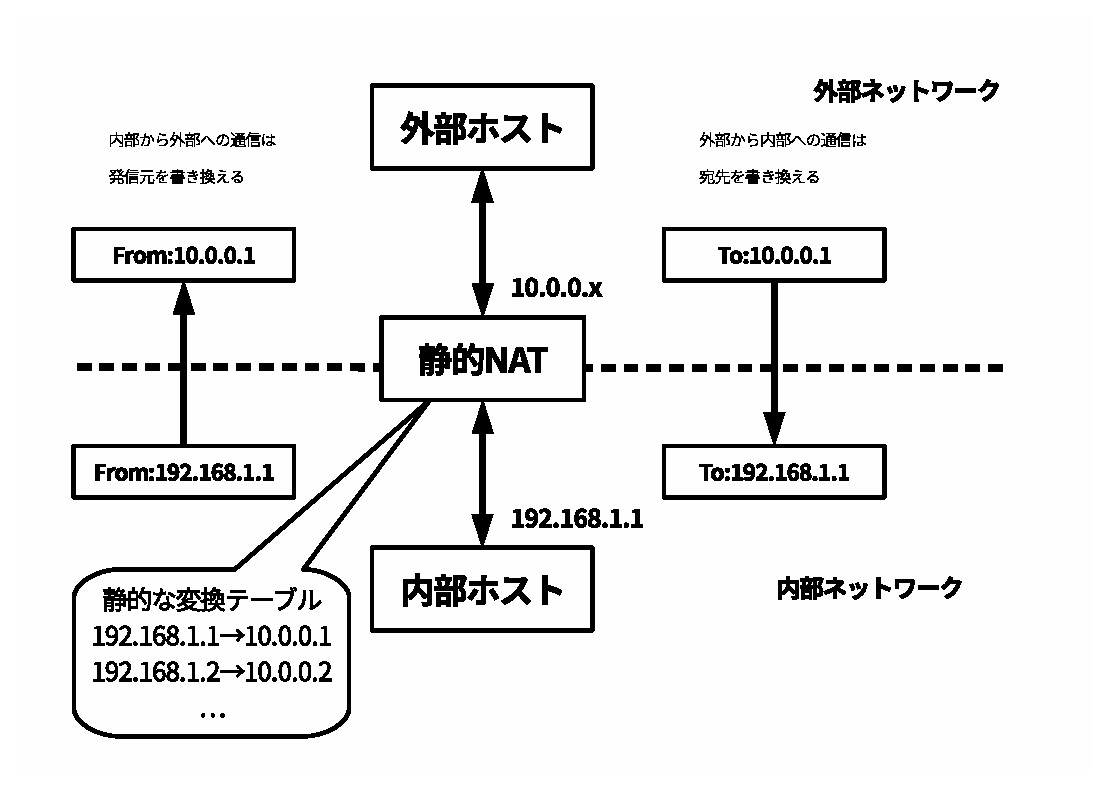
\includegraphics[width=12cm,clip]{draw/fig7.eps}
	\caption{静的NAT}
	\label{fig:static-nat}
\end{figure}

ここまで説明したやり方でIPアドレスを変換することで、LANの内部からインターネットに、任意の通信を送ることができる。同様に、LANの外から、NAL内の、アドレス変換の対象となっているホストへ通信をすることもできる。

この方法を、ネットワークアドレス変換(Network Address Translation)の略で、NATと呼ぶ。また、外部のIPアドレスと内部のIPアドレスを一対一で変換するものを、静的NAT(Static NAT)と呼ぶ。

また、静的NATでは、IPデータグラムのヘッダにある宛先情報情報以外は変換しない。これは、もしトランスポート層の通信をペイロードとして運んでいれば、そのヘッダにある発信元ポート番号、宛先ポート番号等の情報を、積極的に変換しないということである。
トランスポート層のチェックサムの値は、NATの副作用として必要となる処理である。

静的NATの利点は、LAN内部にある、プライベートなアドレスを持つホストと、外部にあるグローバルなアドレスを持つホストが、対等に通信できるということである。この点が、アプリケーション層のプロキシとの最大の違いである。

欠点としては、通信させたいホストの数だけ、グローバルのIPアドレスが必要となることだ。このことを単純に考えれば、直接グローバルのアドレスを割り当てればいいように思える。

では、なぜ直接グローバルのアドレスを割り当てず、静的NATを使うのであろうか。

\subsection{静的NATの背景}
元々、静的NATはどのような使われ方をしていたのだろうか。ここまでは、LANの中のホストがファイブとタイトウに津シンできるようにするため、という説明をしてきた。では何故、わざわざ静的NATをつかうようなやりかたをしたのか。

それは、対象となるホストが、本来LANの中にサービスを提供するためのものである。そのため、一つあるネットワークインタフェイスはLANにつなぐ。そして、外部と通信する場合の方を特例として扱い、静的NAT経由で通信をおこなうというわけだ。

また、サーバファームで静的NATを使うこともある。これは、サーバ間の通信はプライベートなアドレスで行い、外部との通信だけ、NAT経由で行う。このように、ひとつのインタフェイスにひとつのIPアドレスを割り当てて、内部にはグローバルなIPアドレスを意識させずに通信することができる。

\section{動的NAT}

\begin{figure}[htbp]
	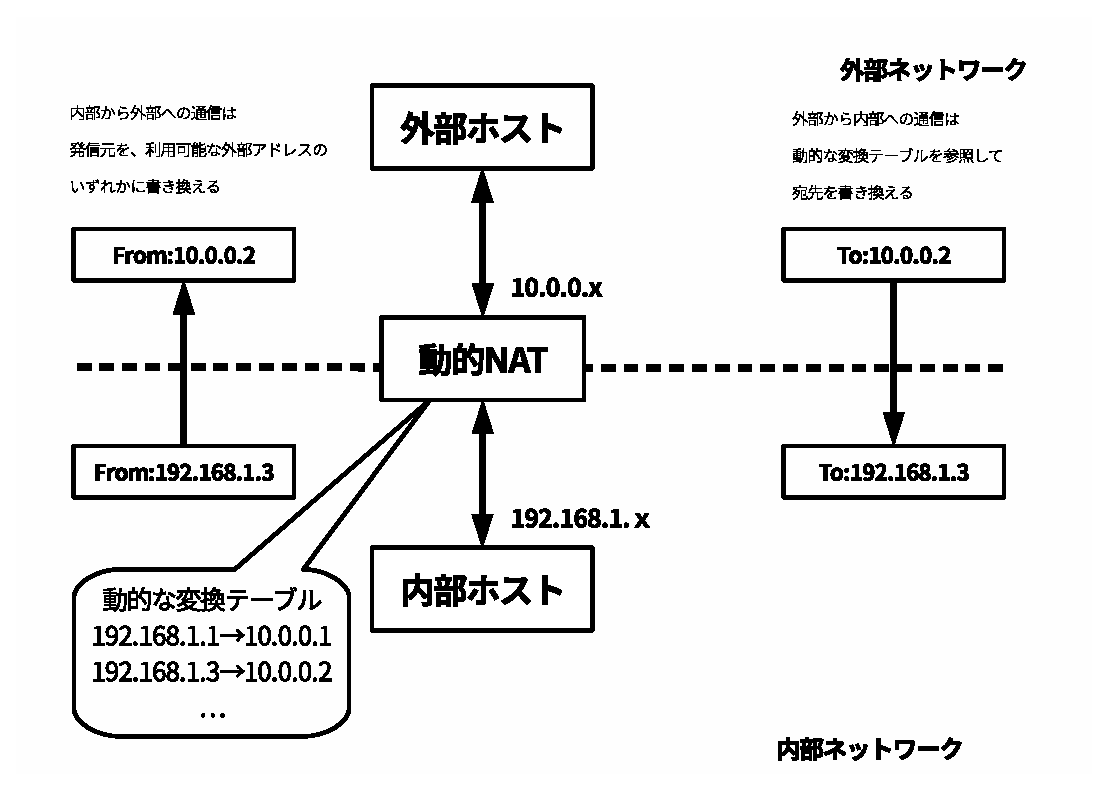
\includegraphics[width=12cm,clip]{draw/fig8.eps}
	\caption{動的NAT}
	\label{fig:dynamic-nat}
\end{figure}

静的なNATがあれば、その対比として動的NATというものが考えられる。では、動的NATとはどんなものであろううか。

動的NATは、インターネットと通信したい内部のホストよりも、グローバルのIPアドレスが少ないときに用いられる。内部から通信のリクエストがある毎に、空いているグローバルIPアドレスがあれば、それと内部のアドレスをマッピングして通信をする。

つまり、毎回の通信で、内部のアドレスと外部のアドレスのマッピングは一定にならない。

誤解されることが多いが、動的NATでは、次章で説明するポート番号の変換は行われないl。IPアドレスをマッピングするだけである。


\subsection{動的NATの問題}

動的NATでは、、毎回の通信で、マッピングされるグローバルIPアドレスは一定しない。そのため、静的NATと異なり、動的NATを介して、外部から内部へのアクセスを行うことはできない。

また、通信毎にIPアドレスを内部ホストで共用する方法なので、TCPのセッションを一定時間維持して、3way Handshakeという比較的重たい処理を減らす、Keepaliveとも相性が悪い。

\subsection{NATのよびかた}
NATは、実装毎にいくつか別の呼び方をされることがある。たとえば、単純にNATと書いたときに、静的NATを指す場合がある。また、メーカによってはMIP(Mappked IP)という呼び方をすることもある。この呼び方の違いは、使用する実装のマニュアルで確認するしかない。

